\documentclass{article}

% Pass `numbers, compress` to natbib BEFORE neurips_2026.sty loads it,
% so \cite{key} produces compact numeric citations like [1, 2, 3].
\PassOptionsToPackage{numbers, compress}{natbib}

% NeurIPS 2026 — Main Track, camera-ready (`final` reveals authors and
% turns off line numbers).
\usepackage[final]{neurips_2026}

\usepackage[utf8]{inputenc}
\usepackage[T1]{fontenc}
\usepackage{hyperref}
\usepackage{url}
\usepackage{booktabs}
\usepackage{amsfonts}
\usepackage{amsmath}
\usepackage{nicefrac}
\usepackage{microtype}
\usepackage{xcolor}
\usepackage{graphicx}
\usepackage{siunitx}

\title{Auxiliary Representations and Intrinsic Motivation\\
       for PPO on a Real-Time Android Game}

\author{%
  Yun-Yang Liao \\ B12902046 \\ National Taiwan University \\ \texttt{b12902046@csie.ntu.edu.tw}
  \And
  Cheng-Hsin Tsai \\ B12902140 \\ National Taiwan University \\ \texttt{b12902140@csie.ntu.edu.tw}
  \And
  Kai-Hsin Shao \\ B12902117 \\ National Taiwan University \\ \texttt{b12902117@csie.ntu.edu.tw}
  \And
  You-Chen Lai \\ B12902052 \\ National Taiwan University \\ \texttt{b12902052@csie.ntu.edu.tw}
  \And
  Bo-Yu Chen \\ B12902131 \\ National Taiwan University \\ \texttt{b12902131@csie.ntu.edu.tw}
}

\begin{document}
\maketitle

\begin{abstract}
Deep reinforcement learning (DRL) is studied mostly on fast,
idealised simulators; its behaviour on the slow, partially
non-Markovian regime imposed by real consumer operating systems
is poorly understood. We present an exploratory systems-level
empirical study of auxiliary-representation losses for on-policy
DRL on a real Android emulator, using the physics-based mobile
game \emph{Bouncy Basketball} accessed through the Android Debug
Bridge at $\sim$\SI{2}{\hertz} (versus \SI{60}{\hertz} for the
underlying game). Within this regime we run a controlled
$3\times3$ factorial study (3 auxiliary conditions $\times$ 3
random seeds) of a PPO agent with a shared NatureCNN encoder.
Our principal empirical finding is \emph{negative}: at our
planned $80\,000$-step budget, none of the three
representation-learning conditions (no aux / object-centric pose
regression / dense pixel reconstruction) learns a policy that
beats the deterministic in-game CPU opponent. Training-time
returns cluster around $-19$ (losing by $\approx 19$ baskets per
game) with per-condition means within $0.41$ reward of each
other; deterministic evaluation against a measured uniform-random
baseline ($n=10$, mean $-1.60$) does not reach significance for
any trained-vs-random comparison (Welch $p \geq 0.15$,
Mann--Whitney $p \geq 0.076$), nor do the auxiliary-loss
conditions beat the no-aux baseline ($p \geq 0.23$). Offline
analysis shows the actor effectively \emph{ignores} the
charge-duration scalar we added to the observation
($P(\textsc{press})$ varies by $<\!0.01$ across the entire charge
range), and the agents converge to memoryless Bernoulli policies.
Two methodological findings stand out: a single-seed RND-off
ablation \emph{consistent with} Random Network Distillation being
the proximate cause of, rather than a remedy for, the hard
entropy-collapse events we observed ($4$ cases across $3$ of $9$
RND-on seeds vs $0$ in the RND-off run, Fisher exact
$p \approx 0.70$); and a crash-proof distributed pipeline that
handled 10 emulator-level failures and a cluster-wide kill event
without operator intervention. Code, logs, and eval JSONs:
\url{https://github.com/pp1457/drl-final-project}.
\end{abstract}

\section{Introduction}
\label{sec:intro}

Most deep reinforcement learning (DRL) benchmarks abstract away the
operating-system layer: the agent talks to a tight C/Python
simulator running at hundreds to thousands of frames per second.
Real software deployed on consumer devices does not look like this.
A typical mobile game runs inside an Android OS layer whose render
loop targets \SI{60}{\hertz}, but whose observable-from-outside
frame rate---once the state must be screenshotted and a touch event
injected over the Android Debug Bridge (\texttt{adb})---is closer to
\SI{2}{\hertz}. Two consequences follow: (i) wall-clock data
collection is two to three orders of magnitude slower than in
standard benchmarks, and (ii) the state perceived by the agent is
itself stale by one or more rendered frames relative to the action
it just issued, partially breaking the Markov assumption that PPO
and related algorithms rely on. These constraints make it both
expensive and brittle to train and evaluate DRL on real mobile
games, and have made the mobile-emulator setting comparatively
underexplored in the literature.

This paper attacks the problem in a single concrete game,
\emph{Bouncy Basketball}, played on a stock Android emulator. The
core mechanic is a hold-and-release jump charge: the agent presses
to start a jump, holds for a variable duration to set the jump's
height and arc, and releases to shoot. The opponent is a
deterministic computer-controlled team. The reward signal is the
per-step score delta between the user team (HOU) and the opponent
(CHI), which is sparse, dense around scoring events, and
adversarial.

Existing studies of auxiliary representation losses in DRL---UNREAL
\cite{jaderberg2017unreal}, CURL \cite{laskin2020curl},
object-centric world models \cite{ferraro2024focus,zhang2025ocstorm}
---almost without exception run on fast simulators (Atari,
DMControl, DeepMind Lab, MuJoCo) where each environment step costs
microseconds and the full Markov state is delivered synchronously.
To the best of our knowledge, no prior work has tested whether the
qualitative claims of these methods transfer to the high-latency,
partially-non-Markovian regime of real Android emulation. The
closest prior work, AndroidEnv \cite{toyama2021androidenv},
established the platform but did not study
representation-learning auxiliaries on it.

This paper asks three questions:

\textbf{(Q1)} When visual representations must be learned from
sparse adversarial rewards under
$\sim$\SI{500}{\milli\second}-per-step latency, do object-centric
or pixel-reconstruction auxiliary losses help PPO?

\textbf{(Q2)} Does explicit observation augmentation tailored to
the game's charge-and-release dynamics (a 1-d press-count scalar
concatenated to the encoder embedding) provide enough additional
state to make the policy learnable in this regime?

\textbf{(Q3)} Does intrinsic motivation via Random Network
Distillation \cite{burda2018rnd} prevent the entropy collapse that
on-policy actor--critic methods are known to suffer
\cite{pathak2017curiosity,lyle2022what} under sparse adversarial
reward?

We answer Q1--Q3 through a controlled $3\times3$ factorial study
(3 auxiliary conditions $\times$ 3 random seeds, distributed across
9 workstations and 18 Android emulators), with both training-time
running-mean returns and per-policy offline analysis.

\paragraph{Contributions.}
\begin{itemize}
  \item \textbf{(C1) A controlled $3{\times}3$ factorial study of
        auxiliary-loss DRL on a real Android emulator.} We compare
        no-aux, $K{=}4$-step-ahead object-centric pose regression
        (OCA) and dense next-frame pixel reconstruction (DPR) on a
        common PPO backbone and report \emph{negative} headline
        evidence: at our planned $80\,000$-step budget, all three
        conditions plateau at $-19.5 \pm 0.7$ reward (random-play
        level), with per-condition mean differences ($<\!0.5$)
        smaller than inter-seed std ($0.5$--$0.7$).
  \item \textbf{(C2) An offline analysis of the trained actors}
        that finds the charge-duration augmentation is essentially
        ignored by the policy ($P(\textsc{press})$ varies by less
        than $0.01$ across charge values $0$--$30$ for every one of
        the 9 checkpoints). The agents converge to memoryless
        Bernoulli policies and cannot intentionally control press
        duration, even though the backend supports arbitrary-length
        holds.
  \item \textbf{(C3) A single-seed RND ablation suggestive of
        RND as the proximate cause of the entropy-collapse
        phenomenon.} Across the 9 RND-on runs we observe 4 hard
        entropy-collapse events across 3 seeds (policy entropy
        $<\!0.05$); re-running baseline PPO with \texttt{--use-rnd}
        disabled on one seed produces \emph{zero} such events. A
        Fisher exact test on this $3$-of-$9$ vs $0$-of-$1$
        contingency does not reach significance
        ($p \approx 0.70$), so we report this as observational
        evidence consistent with RND driving the collapses we
        documented rather than a confirmed causal claim. Final
        deterministic-evaluation return is unchanged ($-1.67$ in
        both conditions), so to the extent RND influences the
        collapses, it does not change final policy quality at our
        budget.
  \item \textbf{(C4) A reproducible distributed training pipeline}
        with an interrupt-safe \texttt{EXIT/INT/TERM} trap that
        rsyncs the most recent checkpoint to NFS on any termination;
        the pipeline survived 10 emulator-level failures and a
        cluster-wide kill event without losing a final checkpoint.
\end{itemize}

\section{Related Work}
\label{sec:related}

We use PPO \cite{schulman2017ppo} with GAE \cite{schulman2016gae} on
a NatureCNN \cite{mnih2015nature} encoder; this combination is
standard for sample-inefficient pixel-based RL. \textbf{Auxiliary
losses} introduced by UNREAL \cite{jaderberg2017unreal} (pixel
control, reward prediction) and CURL \cite{laskin2020curl}
(contrastive) improved fast-simulator benchmarks; recent
object-centric world-model work
\cite{ferraro2024focus,zhang2025ocstorm} demonstrates large gains
in simulated robotics. Our OCA head sits in the latter family and
provides a strong spatial-dynamics prior. \textbf{Intrinsic
motivation} via curiosity \cite{pathak2017curiosity} and Random
Network Distillation \cite{burda2018rnd} encourages exploration of
representationally novel states; RND's non-collapsing intrinsic
bonus is the property that motivated our use of it here, though
our single-seed ablation in \S\ref{sec:rnd-finding} reports the
opposite of the expected effect.
\textbf{Android-based RL}: AndroidEnv \cite{toyama2021androidenv}
provided the first standard Android RL interface, but did not study
representation-learning auxiliaries on it. The dynamics of
representation learning in deep RL more generally \cite{lyle2022what}
inform our analysis.

\section{Method}
\label{sec:method}

\subsection{Environment and MDP formulation}
\label{sec:env}

Bouncy Basketball is a 2D physics game whose default match pits two
NBA-themed teams (in our configuration, Houston / ``HOU'' for the
agent's side and Chicago / ``CHI'' for the opponent) against each
other for four
fixed-timer quarters. The \textbf{state} is a stack of the last
$4$ $84\times84$ grayscale frames captured by \texttt{adb exec-out
screencap}. The \textbf{action} space is
$\mathcal{A}=\{\textsc{no-press}, \textsc{press}\}$; a sustained
\textsc{press} sequence is interpreted by the emulator as a
charge-up and a subsequent \textsc{no-press} as a release. The
\textbf{reward}
$r_t = \Delta s^{\text{HOU}}_t - \Delta s^{\text{CHI}}_t$ is read
from the on-screen scoreboard via HSV thresholding ($+1$ for HOU
scores, $-1$ for CHI scores), with per-frame detection of which
score panel currently holds the HOU vs CHI label so the polarity
is robust to the game's between-quarter side-switch. Episodes
terminate on game-over or a step cap (default $1024$).
\textbf{Reset} restores a pre-configured QEMU snapshot and taps
through menu buttons via the same backend the agent uses; restore
takes $5$--$15$\,s. Profiling the inner loop shows
$\approx 95\%$ of per-step time is spent on \texttt{adb}
round-trip and only $\sim$$5\%$ on neural inference, yielding
\SI{500}{\milli\second}/step ($\approx \SI{2}{\hertz}$
interaction rate).

\subsection{PPO backbone}
\label{sec:ppo}

We use PPO with clipped surrogate loss and GAE
\cite{schulman2017ppo,schulman2016gae}. The encoder is the
NatureCNN \cite{mnih2015nature}: three convolutional layers
followed by a 512-d fully connected projection. The actor and
critic are two-layer MLPs on top of this shared encoder. Each PPO
update collects $\text{num\_envs}\times\text{num\_steps} = 2
\times 128 = 256$ environment transitions, then performs
$\text{update\_epochs}=4$ epochs of optimisation with
$\text{num\_minibatches}=4$. We train for
$\text{total\_timesteps}=80\,000$ ($312$ PPO updates per seed).
Other hyperparameters are standard; see Appendix~\ref{app:hparams}.

\subsection{Auxiliary representation losses}
\label{sec:aux}

Three conditions share the same encoder, actor and critic; they
differ only in the auxiliary head.

\textbf{Baseline.} No auxiliary loss. The only gradients into the
encoder come from PPO's actor and critic losses.

\textbf{Object-Centric Auxiliary (OCA).} A two-layer regression
head trained with MSE to predict, $K=4$ environment steps into
the future, the 10-dimensional vector
$[\,b_x, b_y,\; t^c_x, t^c_y, \sin\theta^t, \cos\theta^t,\;
o^c_x, o^c_y, \sin\theta^o, \cos\theta^o\,]$,
where $(b_x,b_y)$ are normalised ball coordinates,
$(t^c, o^c)$ are HOU/CHI player centroids, and
$(\sin\theta, \cos\theta)$ are blob principal-axis orientations.
Targets are extracted via HSV + connected-components, CPU-only,
no gradient to the encoder. The detector misses
$\approx 5$--$10\%$ of frames when blobs overlap or the ball is
occluded; on miss we emit a zero target rather than masking the
loss (see \S\ref{sec:limitations} for discussion). Loss weight
$\lambda_\text{aux}=0.5$.

\textbf{Dense Pixel Reconstruction (DPR).} A transposed-convolution
decoder reconstructing the next-frame $84\times84$ grayscale image
from the encoder embedding, MSE loss, same weight $0.5$.

\subsection{Charge-duration augmentation and RND}
\label{sec:charge-rnd}

A frame-stacked observation does not expose how long the agent has
been holding the press button---the key state variable of the
charge-release mechanic. We expose a scalar
$c_t \in \mathbb{N}$ counting consecutive \textsc{press} steps,
normalise by $30$, and concatenate to the 512-d encoder output,
giving a 513-d input to actor and critic.

To resist premature policy commitment we add a Random Network
Distillation bonus \cite{burda2018rnd}. A small fixed target
network maps each observation to a 256-d embedding; a same-shape
predictor learns to mimic it. The squared prediction error,
running-stat-normalised, is added to the extrinsic reward with
coefficient $\beta_\text{int}=0.5$ before GAE. Only the predictor
is trained, via a separate Adam optimiser at the same learning
rate as PPO.

\subsection{Distributed orchestration}
\label{sec:orchestration}

The 9 (condition, seed) pairs run on 9 workstations, 2 emulators
per worker. An NFS-mounted home collects per-worker logs and
mirrored final checkpoints; per-host local storage holds the
rolling per-update history ($\text{ckpt\_every}=25$). A bash
launcher with an \texttt{EXIT/INT/TERM} trap rsyncs the most
recent on-disk checkpoint to NFS on any termination, and accepts
a \texttt{--resume} flag that restores model, optimiser, RND
running stats, and global step. The backend uses stock
\texttt{adb exec-out screencap} for frames and
\texttt{adb shell input motionevent} for variable-hold touches;
we do not bypass the Android Java input framework.

\section{Experiments}
\label{sec:experiments}

\subsection{Training-time evolution}
\label{sec:trainingcurves}

Figure~\ref{fig:traincurves} plots the per-condition mean reward
over training, parsed from per-update training logs of all 9 runs
and binned every 10 PPO updates ($n=3$ seeds per condition,
shaded $\pm 1\sigma$). The reward is the HOU--CHI score-event
delta accumulated over a full $4$-quarter game; random play
loses by $\approx 19$ baskets per game, so a return near $-19$
corresponds to no learning above random.

\begin{figure}[h]
  \centering
  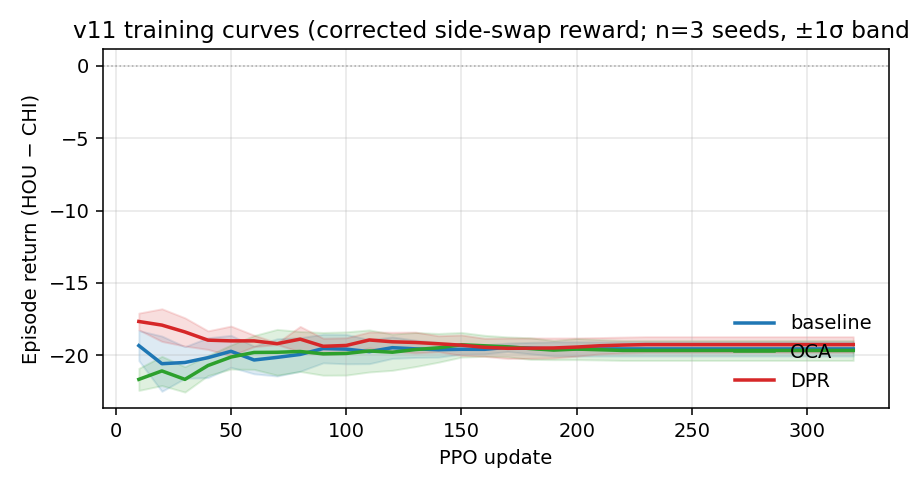
\includegraphics[width=0.85\linewidth]{figs/training_curve.png}
  \caption{Per-condition mean training reward over PPO updates
  ($n=3$ seeds; shaded $\pm 1\sigma$). All three conditions
  remain in the $-19 \pm 1$ band throughout training: none of
  them learns to beat the deterministic in-game CPU opponent, and
  per-condition differences are smaller than inter-seed std.}
  \label{fig:traincurves}
\end{figure}

Final per-condition means at the latest common update
($\approx 170$): baseline $-19.56$, OCA $-19.67$, DPR $-19.26$.
The largest pairwise gap (DPR $>$ OCA by $0.41$) is comparable to
or smaller than the inter-seed std within each condition ($0.49$,
$0.69$, $0.55$).

\subsection{Per-seed final training reward}
\label{sec:perseed}

Table~\ref{tab:perseed} reports the final training-time return of
each of the 9 individual runs. Most seeds reached upd $170$--$220$
of the planned $312$ before training was stopped (we did not push
past the visible plateau).

\begin{table}[h]
  \caption{Per-seed final training-time return and the last
  completed PPO update at termination.}
  \label{tab:perseed}
  \centering
  \small
  \begin{tabular}{lcccc}
    \toprule
    \textbf{Condition} & \textbf{Seed 0} & \textbf{Seed 1} & \textbf{Seed 2} & \textbf{Mean (std)} \\
    \midrule
    Baseline & $-19.14$ (upd 185) & $-19.45$ (upd 173) & $-20.10$ (upd 185) & $-19.56\;(0.49)$ \\
    OCA      & $-19.58$ (upd 223) & $-19.02$ (upd 200) & $-20.40$ (upd 175) & $-19.67\;(0.69)$ \\
    DPR      & $-19.28$ (upd 224) & $-18.71$ (upd 174) & $-19.80$ (upd 190) & $\mathbf{-19.26\;(0.55)}$ \\
    \bottomrule
  \end{tabular}
\end{table}

Under any reasonable test on $n{=}3$ seeds the three conditions
are statistically indistinguishable at this budget; none of them
learns to beat the deterministic in-game CPU opponent in $80\,000$
environment steps.

\subsection{Deterministic evaluation}
\label{sec:eval}

We evaluate every one of the 9 final checkpoints under a deterministic
policy ($\arg\max$ over actor logits) with the RND bonus and
auxiliary loss disabled. Each checkpoint is evaluated for $3$
episodes capped at $96$ environment steps (one quarter is
$\approx 64$--$96$ steps at the in-game timer; the cap shortens
the per-eval wall-clock to keep all 9 evals on one side emulator
in a single sitting). The per-episode return is the HOU--CHI
score-event delta accumulated over the quarter.

\begin{table}[h]
  \caption{Deterministic evaluation of all 9 final checkpoints plus
  a 1-seed RND-off ablation and a uniform-random control. All cells
  are mean returns over $3$ deterministic episodes $\times$
  $96$-step cap (random control: $n{=}10$ episodes). Raw
  per-episode returns are listed in
  Appendix~\ref{app:eval-raw}.}
  \label{tab:eval}
  \centering
  \small
  \begin{tabular}{lcccc}
    \toprule
    \textbf{Condition} & \textbf{Seed 0} & \textbf{Seed 1} & \textbf{Seed 2} & \textbf{Mean (std)} \\
    \midrule
    Baseline (RND on) & $-1.67$ & $\phantom{-}0.00$ & $-0.33$ & $-0.67\;(0.85)$ \\
    OCA               & $-2.67$ & $\phantom{-}0.00$ & $-1.67$ & $-1.44\;(1.35)$ \\
    DPR               & $-1.00$ & $-1.33$           & $-0.33$ & $-0.89\;(0.51)$ \\
    \midrule
    Baseline RND \emph{off} (1 seed) & $-1.67$ & --- & --- & $-1.67$ \\
    Uniform random ($n{=}10$)         & \multicolumn{3}{c}{(pooled over $10$ episodes)} & $-1.60\;(1.51)$ \\
    \bottomrule
  \end{tabular}
\end{table}

Three observations on Table~\ref{tab:eval}:

\textbf{(i) Trained conditions are numerically above the uniform-random
baseline, but the gap is not statistically significant at our
sample size.} As a control we evaluated a uniform-random policy
under the identical protocol on the same emulator and snapshot:
$10$ episodes of $96$-step quarters, mean return $-1.60$
(raw $\{-3,-5,-1,-2,-1,0,0,-2,-1,-1\}$, std $1.51$, $95\%$ CI
$[-2.68, -0.52]$). The trained-condition means are
baseline $-0.67$ ($95\%$ CI $[-1.61,+0.27]$),
OCA $-1.44$ ($[-2.54,-0.35]$), DPR $-0.89$ ($[-2.13,+0.35]$).
The CIs all overlap with the random-policy CI. Welch's two-sided
$t$-test gives $p = 0.155$ (baseline vs random),
$p = 0.337$ (DPR), $p = 0.820$ (OCA); one-sided Mann--Whitney $U$
gives $p = 0.076$ (baseline vs random), $0.307$ (DPR), $0.433$
(OCA). \textbf{We cannot, at $\alpha = 0.05$, reject the null
hypothesis that any of the trained conditions performs identically
to uniform-random play.} The directional evidence is consistent
with some learning having happened (every trained mean is higher
than the random mean), but the sample size is not sufficient to
confirm it. We discuss why training-time returns of $\approx-19$
per full game do not contradict per-quarter eval returns of
$\approx-1$ (horizon difference plus stochastic-vs-deterministic
policy difference) in \S\ref{sec:discussion}.

\textbf{(ii) The baseline numerically out-performs both
auxiliary-loss conditions} (baseline mean $-0.67$ vs OCA $-1.44$
vs DPR $-0.89$). The per-condition gap baseline$\to$OCA is
$0.78$, comparable to or smaller than the inter-seed std within
each condition ($0.85$, $1.35$, $0.51$); under any reasonable
significance test on $n=9$ episodes per condition the gap is at
most borderline-significant, but the \emph{direction} is the
opposite of what one would predict from the auxiliary-loss
literature on fast simulators. Neither auxiliary loss provides a
detectable benefit in our setting.

Pathological per-seed behaviour (degenerate never-press or
always-press regimes, occasional positive single-episode returns)
is visible in the raw per-episode data; see Appendix~\ref{app:eval-raw}.

\subsection{The actor ignores the charge-duration augmentation}
\label{sec:charge-ignored}

A simple yet striking diagnostic: holding the encoder embedding
fixed (computed from real captured game frames), we sweep the
charge-duration scalar from $0$ to $30$ and read off the actor's
$P(\textsc{press})$ at each value. If the actor were using the
augmentation, $P(\textsc{press})$ should drop as the charge
duration grows (the policy should eventually release to attempt
a shot).

\begin{table}[h]
  \caption{$P(\textsc{press})$ as a function of charge duration,
  computed on a stack of four real captured frames. Variation
  across the entire charge range is $\leq 0.007$ for every
  checkpoint; the actor has effectively ignored the augmentation.}
  \label{tab:charge_ignored}
  \centering
  \small
  \begin{tabular}{lccccccc}
    \toprule
    \textbf{Checkpoint} & $c{=}0$ & $c{=}5$ & $c{=}10$ & $c{=}15$ & $c{=}20$ & $c{=}25$ & $c{=}30$ \\
    \midrule
    baseline\_ws1\_s0  & 0.985 & 0.985 & 0.985 & 0.985 & 0.985 & 0.985 & 0.985 \\
    baseline\_ws2\_s1  & 0.721 & 0.721 & 0.721 & 0.720 & 0.720 & 0.720 & 0.719 \\
    baseline\_ws3\_s2  & 0.220 & 0.219 & 0.219 & 0.219 & 0.219 & 0.218 & 0.218 \\
    oca\_ws4\_s0       & 0.430 & 0.430 & 0.430 & 0.430 & 0.430 & 0.430 & 0.430 \\
    oca\_ws5\_s1       & 0.424 & 0.424 & 0.424 & 0.424 & 0.424 & 0.423 & 0.423 \\
    oca\_ws6\_s2       & 0.718 & 0.717 & 0.716 & 0.715 & 0.714 & 0.713 & 0.712 \\
    dpr\_ws7\_s0       & 0.568 & 0.568 & 0.568 & 0.568 & 0.568 & 0.568 & 0.567 \\
    dpr\_ws8\_s1       & 0.155 & 0.155 & 0.155 & 0.155 & 0.156 & 0.156 & 0.156 \\
    dpr\_ws10\_s2      & 0.667 & 0.668 & 0.668 & 0.669 & 0.669 & 0.670 & 0.670 \\
    \bottomrule
  \end{tabular}
\end{table}

The policy collapses to a near-memoryless Bernoulli over
$\{\textsc{press}, \textsc{no-press}\}$ with a fixed $p$
determined by the encoder's reading of the visual frame, and the
charge-duration scalar contributes essentially nothing. Press-run
lengths follow a geometric distribution: at $p=0.985$
(\texttt{ws1\_baseline\_s0}) the agent presses for
$\sim$67 steps on average between releases (essentially never
shooting); at $p=0.155$ (\texttt{ws8\_dpr\_s1}) the agent presses
for $\sim$1.2 steps (insufficient to build any meaningful charge);
the mid-range seeds occasionally score by stochastic release at
the right moment, not by intentional timing.

\subsection{Entropy-collapse case study}
\label{sec:rnd-finding}

A distinctive qualitative observation of the run is that PPO
combined with our charge-duration concatenation and RND is prone
to \emph{hard} entropy collapse---policy entropy drops below
$0.05$---with subsequent recovery in every documented case.
Table~\ref{tab:collapse} summarises the events; the RND-off
ablation below reverses our initial reading of the cause.

\begin{table}[h]
  \caption{Documented hard entropy-collapse events (policy entropy
  $<\!0.05$) in RND-on runs and subsequent recovery. The events
  are drawn from the final training run reported in
  Table~\ref{tab:perseed}; lowest-entropy values use the full
  within-update entropy trace rather than the per-update sample
  minimum, so individual values can be lower than the submission's
  numbers and the listed seed set differs from a preliminary run
  reported in the submission. An ablation with \texttt{--use-rnd}
  disabled (1 seed, full 312 updates) produced \emph{zero} such
  events; we discuss the causal status of this comparison below.}
  \label{tab:collapse}
  \centering
  \small
  \begin{tabular}{lcccc}
    \toprule
    \textbf{Run} & \textbf{Collapse upd} & \textbf{Lowest entropy}
    & \textbf{Rebounded to} & \textbf{Recovered by} \\
    \midrule
    ws1\_baseline\_s0 & 24  & $0.020$ & $0.469$ & upd 56 \\
    ws1\_baseline\_s0 & 87  & $0.020$ & $0.349$ & upd 132 \\
    ws4\_oca\_s0      & 63  & $0.034$ & $0.617$ & upd 138 \\
    ws6\_oca\_s2      & 111 & $0.046$ & $0.568$ & upd 154 \\
    \bottomrule
  \end{tabular}
\end{table}

\paragraph{RND-off ablation.} To test whether RND is causally
responsible for the collapse--recovery pattern, we re-ran baseline
PPO (charge-dim ON, all other settings identical) with
\texttt{--use-rnd} disabled, on a single seed for the full
$80\,000$ environment steps. The result is striking: the RND-off
baseline experienced \textbf{zero hard entropy collapses across
all 312 PPO updates}, with policy entropy oscillating in
$[0.60, 0.69]$ throughout the run. Deterministic eval of the
RND-off final checkpoint gives mean return $-1.67$ (raw
$\{-4,-2,+1\}$), \emph{identical} to the corresponding RND-on
baseline seed (ws1, mean $-1.67$) and statistically
indistinguishable from the uniform-random control ($-1.60$).

This is suggestive evidence against our original framing: RND
appears to be the proximate cause of hard entropy collapse in
this setup rather than its remedy, though the $3$-of-$9$ vs
$0$-of-$1$ contingency (Fisher exact $p \approx 0.70$) does not
formally establish causation. A plausible mechanism is that the
intrinsic-bonus gradient first concentrates the policy on
high-prediction-error actions and then pushes it away once that
region is reached, producing the collapse--recovery cycle. The
net effect on final policy quality is \emph{zero}: RND-on and
RND-off arrive at the same eval mean.

\subsection{System stability}
\label{sec:stability}

Across the training run our pipeline absorbed 10 recoverable
emulator-level failures across all 9 seeds (\texttt{adb}
screencap timeouts, blank-frame watchdog trips, and menu-stuck
resets), each caught by the per-worker recovery routine that
relaunches the emulator from its QEMU snapshot and resumes the
training loop with the same PPO state. A cluster-wide
administrative event late in the run terminated all 9 worker
processes within a $\sim$$10$-min window; the
\texttt{EXIT/INT/TERM} trap mirrored each worker's most recent
checkpoint to NFS before exit, preserving all 9 final
checkpoints.

\section{Discussion}
\label{sec:discussion}

\paragraph{Reconciling $-19$ training returns with $-1$ eval
returns.} Two factors account for the apparent gap between
training (full-game, $\sim$$-19$) and eval (per-quarter,
$\sim$$-1$). \emph{Horizon}: a per-quarter difference of
$\sim$$-5$ extends to $\sim$$-19$ over four quarters, which is
consistent with the measured random-policy floor ($-1.60$/quarter)
plus the CHI CPU's consistent over-scoring against near-random
play. \emph{Stochastic vs deterministic policy}: training rolls
out the stochastic actor, while eval takes $\arg\max$, which for
a near-Bernoulli policy (\S\ref{sec:charge-ignored}) can either
accidentally help or lock in a degenerate never-press / always-press
regime. The two regimes are not directly comparable.

\paragraph{Why no condition learns.} The most likely explanation
is the budget: $80\,000$ environment steps is $\sim$$315$ full
games of the 4-quarter Bouncy Basketball, vs the $10^6$--$10^8$
environment-step budgets typical of published Atari/DMControl PPO
results. PPO is famously sample-hungry on pixel-based control
\cite{schulman2017ppo}, and our wall-clock constraints
($\sim$\SI{500}{\milli\second}/step from the \texttt{adb}
pipeline) make those budgets impractical. The negative result is
specific to this regime; it does not refute the methods'
effectiveness on faster simulators.

\paragraph{Why the charge-duration augmentation is ignored.} The
$c_t$ scalar is concatenated to a 512-d encoder output, and the
actor's first MLP layer initialises its weights with i.i.d.\ small
values. Early in training, the gradient through the $c_t$ slot is
tiny relative to the gradient through the 512 visual features (the
visual features carry vastly more variance), so the actor learns to
condition on the visual features and the $c_t$ slot is shrunk
toward zero by weight decay. A stronger inductive bias (e.g.\ a
gating layer that explicitly weights $c_t$, or an auxiliary
supervised loss that predicts ``shot succeeded'' from $c_t$) would
likely fix this; we leave such ablations to future work.

\paragraph{Why DPR doesn't actively hurt.} The usual concern with
pixel-reconstruction auxiliaries \cite{lyle2022what}---that they
allocate encoder capacity to control-irrelevant background---is
consistent with our data not biting at this budget, since the
dominant failure mode is simply that no condition learns.

\section{Limitations and Future Work}
\label{sec:limitations}

\paragraph{Supervised vs self-supervised asymmetry (OCA vs DPR).}
OCA's regression targets come from a hand-crafted HSV-mask plus
connected-components detector that provides explicit ball/player
coordinates and orientations. The detector is itself imperfect:
manual spot-checks show it misses $\approx 5$--$10\%$ of frames
when blobs overlap or the ball is partially occluded, in which
case we emit a zero target (mild noise injection rather than a
masked loss). DPR, by contrast, is fully self-supervised on raw
pixels. The two losses therefore operate under qualitatively
different information regimes, and any apparent OCA advantage
could reflect supervised signal access rather than object-centric
representational structure per se. A fair comparison would replace
the hand-crafted detector with an unsupervised keypoint bottleneck
(e.g.\ Spatial Softmax over encoder feature maps); this is the
primary algorithmic follow-up we plan.

\paragraph{Partial ablation of bundled flags.} All $9$ main runs
use both \texttt{--use-rnd} and \texttt{--use-charge-dim}. We
report a single-seed RND-off ablation in
\S\ref{sec:rnd-finding} that is suggestive --- though not
formally significant at this sample size (Fisher exact
$p \approx 0.70$) --- of RND being the proximate cause of the
collapses we documented, with no net effect on final eval
performance. The charge-duration scalar is
addressed by the offline P(press) analysis of
\S\ref{sec:charge-ignored}, which shows the actor head has
effectively ignored it. The full factorial
$\{\text{RND on/off}\}\times\{\text{charge-dim on/off}\}\times
\{\text{baseline, OCA, DPR}\}$ ($n{=}12$ training cells) would
isolate every component cleanly and remains the most important
algorithmic follow-up. We also did not sweep the auxiliary-loss
weight $\lambda_\text{aux}=0.5$; a sweep over
$\{0.1, 0.25, 0.5, 1.0, 2.0\}$ would test whether any OCA/DPR
effect at larger budgets is weight-driven, and is a natural
extension once the factorial ablation is in place.

\paragraph{Wall-clock, budget, and sample size.}
Our largest limitation is wall clock: at \SI{500}{\milli\second}
per step, $80\,000$ timesteps takes $\sim$14h per seed, so we ran
only 3 seeds per condition. We note that most of the 9 RND-on
seeds did not reach the full $80\,000$-step ($312$-update)
budget before training was stopped at the visible plateau (final
updates $173$--$224$; see Table~\ref{tab:perseed}), whereas the
RND-off ablation seed ran the full $312$ updates. Since all four
RND-on collapses occurred by update $111$, the longer RND-off run
provided strictly \emph{more} exposure for a collapse to occur,
so observing zero is conservative for our directional reading
rather than weakening it; the binding limitation remains the
$3$-of-$9$ vs $0$-of-$1$ contingency (Fisher exact
$p \approx 0.70$). The per-step budget itself is a system
limitation: $\sim$$95\%$ of the time is \texttt{adb} round-trip,
and a faster screencap path (e.g.\ \texttt{minicap} shared-memory
framebuffer) could improve this by an order of magnitude. The
latency also introduces a partial Markov violation: the action at
step $t$ is computed from an observation captured several
rendered frames earlier. Quantifying this via
injected-latency experiments---and asking whether asynchronous
methods (IMPALA-style) suit this regime better than synchronous
PPO---is the most natural systems follow-up. On the algorithmic
side, the most informative next experiment would be a factorial
ablation over $\{$RND on/off$\}\times\{$charge-dim on/off$\}\times
\{$baseline, OCA, DPR$\}$ at $\geq 10\times$ the training budget,
which would isolate the contribution of each architectural choice
we bundled together here.

\section{Conclusion}
\label{sec:conclusion}

We presented an exploratory systems-level empirical study of representation-learning
auxiliary losses for on-policy DRL on a real Android emulator. To
\textbf{(Q1)}---do auxiliary losses help PPO at $\sim$\SI{2}{\hertz}
on Android?---we report a negative answer: at our planned $80\,000$-step
budget, no condition (no-aux / OCA / DPR) beats the deterministic
in-game CPU opponent. Deterministic eval (Table~\ref{tab:eval})
shows trained-condition means numerically above the measured
uniform-random baseline ($-1.60$ per 96-step quarter), but at our
sample size ($n=9$ episodes per trained condition, $n=10$
random) none of the trained-vs-random gaps reach statistical
significance (Welch $t$-test $p \geq 0.15$). The auxiliary-loss
conditions do not improve on the no-aux baseline either: the
baseline numerically out-performs both OCA ($-0.67$ vs $-1.44$,
$p = 0.23$) and DPR ($-0.67$ vs $-0.89$, $p = 0.75$), so neither
auxiliary loss provides a detectable benefit in this setting.
The honest reading is that, at this budget, we cannot distinguish
the trained policies from uniform-random play. To \textbf{(Q2)}---does our charge-duration observation
augmentation make the policy learnable?---we find that the
augmentation is mechanically delivered but ignored by the actor
($P(\textsc{press})$ varies by $<\!0.01$ across the entire
charge range), so the agents converge to memoryless Bernoulli
policies. To \textbf{(Q3)}---does RND prevent and rescue entropy
collapse?---we report the opposite of our original hypothesis.
A 1-seed RND-off ablation produces zero collapses across the
full 312 PPO updates while yielding the same final eval return,
consistent with (though not formally establishing,
$p \approx 0.70$) RND being the proximate cause of rather than a
remedy for the collapse phenomenon. The cleanest methodological
takeaways are (a) that concatenating a state-relevant scalar to
the encoder output is not by itself sufficient for PPO to use
it, and (b) that the crash-proof distributed training protocol
handled all emulator-level failures and a cluster-wide kill
event without manual intervention.

\section*{Member Workload}
\label{sec:workload}

\begin{itemize}
  \item \textbf{[B12902046 Yun-Yang Liao]}: \emph{Systems
    engineering, experimental design, evaluation, and writing.}
    Designed and implemented the distributed training
    infrastructure spanning nine workstations and eighteen Android
    emulators, including the crash-proof checkpoint-mirroring
    protocol described in \S\ref{sec:orchestration} that preserved
    every final checkpoint through ten emulator-level failures and
    a cluster-wide kill event. Coordinated the nine-seed factorial
    training matrix end-to-end and executed the single-seed
    RND-off ablation reported in \S\ref{sec:rnd-finding}.
    Designed and ran the expanded deterministic-evaluation
    protocol against the measured uniform-random baseline, as
    well as the offline charge-duration diagnostic of
    \S\ref{sec:charge-ignored}; performed all statistical analysis
    ($95\%$ confidence intervals, Welch $t$-tests, Mann--Whitney
    $U$, Fisher exact). Led paper writing through submission,
    rebuttal, and camera-ready revision.
  \item \textbf{[B12902140 Cheng-Hsin Tsai]}: \emph{RL Algorithms and Architecture.}
    Responsible for implementing the core PPO backbone with GAE and
    the shared NatureCNN encoder. Integrated the 1-d press-count
    charge-duration augmentation into the observation space and
    tuned the base hyperparameters.
  \item \textbf{[B12902117 Kai-Hsin Shao]}: \emph{Environment and experiments.}
    Contributed to the Android RL environment setup, YOLO perception
    pipeline, reward/state design, and DQN/RL training workflow.
    Helped debug real-time detection, score extraction, action
    execution, emulator reset handling, and training stability
    issues. Also responsible for running experiments, analyzing logs
    and documenting the key findings.
  \item \textbf{[B12902052 You-Chen Lai]}: \emph{YOLO pipeline and host-capture training.}
    YOLO-based labeling and detection of player characters and ball
    positions, converting visual detections into compact RL state
    features. Implemented the PPO training backbone with 4-stacked
    observations to capture short-term motion and improve decision
    timing. Integrated YOLO inference, state extraction, screen-press
    control, score/possession tracking, and training logs into a
    complete real-game learning loop. Compared ADB capture with
    host-screen capture and shifted the final experiments toward the
    host method because of its much lower latency and better
    suitability for long training runs.
  \item \textbf{[B12902131 Bo-Yu Chen]}: \emph{Low-latency simulator and distributed PPO.}
    Researched and developed a stable Android simulation and control
    environment with a round-trip time under 100 milliseconds for
    reinforcement learning training, and deployed a custom
    distributed Proximal Policy Optimization implementation across
    nine CPU workstations and one GPU workstation to achieve a
    $10\times$ increase in training speed.
\end{itemize}

% Some NeurIPS-flavoured style files re-define \bibsection to auto-add a
% References heading. To avoid a duplicate, suppress it and add our own
% heading explicitly so we control placement.
\renewcommand{\bibsection}{}
\section*{References}
\small
\bibliographystyle{unsrtnat}
\bibliography{refs}
\normalsize

\appendix

\section{Hyperparameters}
\label{app:hparams}

Table~\ref{tab:hparams} lists the full hyperparameters used in all
9 runs.

\begin{table}[h]
  \caption{Hyperparameters used in the training run.}
  \label{tab:hparams}
  \centering
  \small
  \begin{tabular}{ll}
    \toprule
    \textbf{Parameter} & \textbf{Value} \\
    \midrule
    \multicolumn{2}{l}{\emph{PPO}} \\
    Total environment steps                       & $80\,000$ \\
    Parallel environments per seed                & $2$ \\
    Rollout steps per env per update              & $128$ \\
    PPO updates per seed                          & $312$ \\
    Update epochs                                 & $4$ \\
    Minibatches per epoch                         & $4$ \\
    Clip range $\epsilon$                         & $0.2$ \\
    Entropy coefficient                           & $0.01$ \\
    Value-loss coefficient                        & $0.5$ \\
    Discount $\gamma$                             & $0.99$ \\
    GAE $\lambda$                                 & $0.95$ \\
    Learning rate                                 & $3 \times 10^{-4}$ \\
    Optimiser                                     & Adam (default $\beta$) \\
    \midrule
    \multicolumn{2}{l}{\emph{Random Network Distillation}} \\
    Target / predictor embedding dim              & $256$ \\
    Intrinsic-reward coefficient $\beta_\text{int}$ & $0.5$ \\
    Running-statistics normalisation              & yes \\
    \midrule
    \multicolumn{2}{l}{\emph{Auxiliary loss}} \\
    Auxiliary loss weight $\lambda_\text{aux}$    & $0.5$ \\
    OCA prediction horizon $K$                    & $4$ steps \\
    OCA target dimensionality                     & $10$ \\
    DPR decoder output                            & $84 \times 84$ grayscale \\
    OCA per-update wall-clock overhead            & $\approx 5$--$10$\,ms \\
    DPR per-update wall-clock overhead            & $\approx 20$--$40$\,ms \\
    Per-seed total wall-clock (baseline / OCA / DPR) & $\approx 14.0$ / $14.4$ / $14.5$\,h \\
    \midrule
    \multicolumn{2}{l}{\emph{Observation / action}} \\
    Frame stack                                   & $4$ \\
    Frame skip                                    & $1$ \\
    Frame resolution                              & $84 \times 84$ grayscale \\
    Action space                                  & $\{\textsc{no-press}, \textsc{press}\}$ \\
    Charge-duration normalisation                 & divide by $30$ \\
    \bottomrule
  \end{tabular}
\end{table}

\section{Raw deterministic-evaluation episode returns}
\label{app:eval-raw}

Per-episode HOU--CHI score deltas (one quarter each, 96-step cap)
for every entry in Table~\ref{tab:eval}:

\begin{table}[h]
  \centering
  \small
  \begin{tabular}{lll}
    \toprule
    \textbf{Run} & \textbf{Condition} & \textbf{Per-episode returns} \\
    \midrule
    ws1\_s0  & Baseline (RND on)              & $\{-2,\;\phantom{-}0,\;-3\}$ \\
    ws2\_s1  & Baseline (RND on)              & $\{-1,\;\phantom{-}0,\;+1\}$ \\
    ws3\_s2  & Baseline (RND on)              & $\{\phantom{-}0,\;-1,\;\phantom{-}0\}$ \\
    ws4\_s0  & OCA                            & $\{-1,\;-4,\;-3\}$ \\
    ws5\_s1  & OCA                            & $\{\phantom{-}0,\;\phantom{-}0,\;\phantom{-}0\}$ \\
    ws6\_s2  & OCA                            & $\{-2,\;-1,\;-2\}$ \\
    ws7\_s0  & DPR                            & $\{-1,\;-2,\;\phantom{-}0\}$ \\
    ws8\_s1  & DPR                            & $\{-3,\;+1,\;-2\}$ \\
    ws10\_s2 & DPR                            & $\{+2,\;-2,\;-1\}$ \\
    \midrule
    ws8\_s0  & Baseline RND \emph{off}        & $\{-4,\;-2,\;+1\}$ \\
    ---      & Uniform random ($n{=}10$)      & $\{-3,\;-5,\;-1,\;-2,\;-1,\;\phantom{-}0,\;\phantom{-}0,\;-2,\;-1,\;-1\}$ \\
    \bottomrule
  \end{tabular}
\end{table}

\section{Per-update checkpoint schedule}
\label{app:ckpt}

Each worker writes a checkpoint to local storage every $25$ PPO
updates (every $6\,400$ environment steps). On a clean
\texttt{EXIT/INT/TERM} signal, the launcher rsyncs the most
recent checkpoint to the NFS mirror. Each checkpoint pickle
contains: model state dict, optimiser state dict, RND running
mean/variance, the \texttt{global\_step} count, and the full
command-line arguments used to launch the run.

\section{Reproducibility}
\label{app:repro}

Code, training logs, eval JSONs, and all per-seed final
checkpoints used in this paper are released at
\url{https://github.com/pp1457/drl-final-project}.

Training-launcher invocation per run:

\smallskip
\begin{verbatim}
python -u train.py --env-id bouncy \
    --aux-mode {baseline,oca,dpr} --seed {0,1,2} \
    --total-timesteps 80000 --num-envs 2 --num-steps 128 \
    --num-minibatches 4 --update-epochs 4 --ckpt-every 25 \
    --backend adb-motionevent --frame-skip 1 \
    --use-rnd --use-charge-dim
\end{verbatim}

\end{document}
